\chapter{Geometry}

Pixels in the image plane have a direct mapping to the position of the camera in the real world. When we use the approximation of the image we might lose some relevant pices of information such as the depth of the objects in the scene or the speed of objects, which will appear slower the further they are from the camera. 

In this chapter we will introduce the basic concepts of geometry that will allow us to understand the relationship between the camera and the real world.

Typically we represent a point (pixel) as a set of coordinates:

\[ P = [ x, y ]^t = \begin{bmatrix} x \\ y \end{bmatrix}\]

Often convenient to use homogeneous coordinates:
\[ P = [ x, y ]^t = [sx, sy, s]\]

Where \( s \) is a scaling factor, commonly set to 1.0, this will help us when doing transformations.

\[ P = [ x, y ]^t = [x, y, 1]\]

Sometimes we can also omit the " \(^t\) " and write the coordinates as a row vector.

\section{Affine Transformations}

Now formally the pixel is a vector so in general we can apply all the kind of transofmations we want, which usually turn out to be combinations of summations and multiplications. 
The most common transformations are:

\begin{itemize} 
    \item Scaling 
    \item Translation 
    \item Rotation 
    \item Combinations of the above 
\end{itemize}

\subsection{Scaling}

In scaling we take one point or a set of points and we transform them by a multiplaying factor.

\[
\begin{bmatrix}
    x' \\
    y'
    \end{bmatrix}
    =
    \begin{bmatrix}
    c & 0 \\
    0 & c
    \end{bmatrix}
    \begin{bmatrix}
    x \\
    y
    \end{bmatrix}
\]

\begin{figure}[ht]
    \centering
    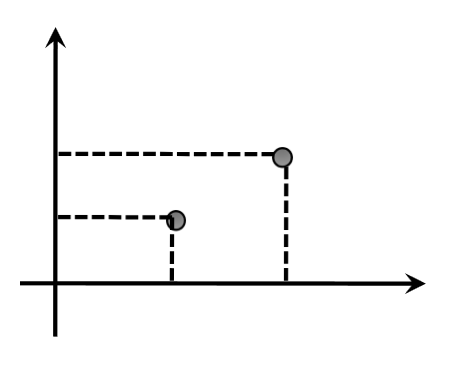
\includegraphics[width=0.3\textwidth]{Figures/scaling.png}
    \caption{Scaling}
    \label{fig:scaling}
\end{figure}

This is a very simple transformation, it can happen that we have not a single coefficient \(c\) but different scaling factors for the different axis.
\[
\begin{bmatrix}
    x' \\
    y'
    \end{bmatrix}
    =
    \begin{bmatrix}
    c_x & 0 \\
    0 & c_y
    \end{bmatrix}
    \begin{bmatrix}
    x \\
    y
    \end{bmatrix}
\]

\subsection{Rotation}

Rotation is the result of applying a rotation angle to the coordinate points, if we go back to the trigonomety we can see that we can use the sine and cosine information of the angle \(\theta\) and we can imagine that if we are rotating a unit vector, the coordinates of the new vector will be the sine and cosine of the angle.

\begin{figure}[ht]
    \centering
    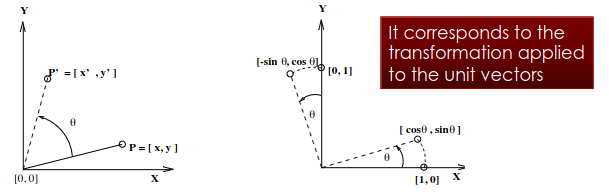
\includegraphics[width=0.75\textwidth]{Figures/rotation.png}
    \caption{Rotation}
    \label{fig:rotation}
\end{figure}

For instance we can see on the horizontal unit vector how the \(x\) gets reduced while a \(y\) component appears correspondin to the sine of the angle.

By the time we have a point that's been shifter by a certain amount \(\theta\), saying that the points rotates equals to keeping the point fixed and rotating the coordinate system by the same amount. The resulting operation that we have in our matrix is the multiplication of the point with the transformation of the unit vectors.

\[
    \begin{bmatrix}
        x' \\
        y'
        \end{bmatrix}
        =
        \begin{bmatrix}
        \cos\theta & -\sin\theta \\
        \sin\theta & \cos\theta
        \end{bmatrix}
        \begin{bmatrix}
        x \\
        y
        \end{bmatrix}
        =
        \begin{bmatrix}
        x \cos\theta - y \sin\theta \\
        x \sin\theta + y \cos\theta
        \end{bmatrix}    
\]

Both scaling and rotation can be constructed using a simple 2 by 2 matrix.
\subsection{Translation}

A translation is simply a shift of the points of our objects into new coordinates.
Just like we can think of rotation as a change in the coordinate system, we can think of translation as a change in the origin of the coordinate system.

If we apply a displacenent vector it's the same as moving the origin of the coordinate system to the new point and we can model this easily:

\( D([x, y]) = [x + x_0, y + y_0] \)

At this point we can't use anymore a 2 by 2 matrix because we have to introduce the two operators \( x_0 \) and \( y_0 \) that are not part of the matrix. 

\[
    \begin{bmatrix}
        x' \\
        y' \\
        \end{bmatrix}
        =
        \begin{bmatrix}
        1 & 0  \\
        0 & 1  \\
        \end{bmatrix}
        \begin{bmatrix}
        x \\
        y \\
        \end{bmatrix}
        +
        \begin{bmatrix}
            x_0 \\
            y_0 \\
        \end{bmatrix}
\]

The new coordinates are nothing but a multiplication of a scaling matrix of facor 1.0 by the coordinates \(x, y\) and then the addition of the translation vector.


To bring the displacement vector inside the matrix we can use the homogeneous coordinates, we can add a third coordinate to the vector and then we can multiply the matrix by the vector.

\[
    \begin{bmatrix}
        x' \\
        y' \\
        1
        \end{bmatrix}
        =
        \begin{bmatrix}
        1 & 0 & x_0 \\
        0 & 1 & y_0 \\
        0 & 0 & 1
        \end{bmatrix}
        \begin{bmatrix}
        x \\
        y \\
        1
        \end{bmatrix}
        =
        \begin{bmatrix}
        x + x_0 \\
        y + y_0 \\
        1
        \end{bmatrix}
\]


\subsection{Rotation, scaling and translation}

Our goal is to be able to map what's happening in the real world to the image plane, we can do this by applying a series of transformations, overall we need to deal with at least 4 parameters:
\begin{itemize} 
    \item One rotation angle (1 parameter)
    \item One scaling factor (1 parameter)
    \item A translation vector (2 parameters)
\end{itemize}

\({}^w P_j = D_{x0,y0} S_s R_\theta {}^i P_i\)


\begin{figure}[ht]
    \centering
    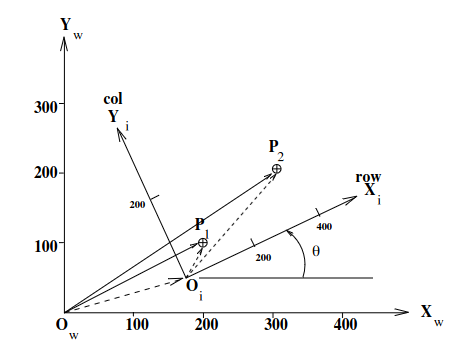
\includegraphics[width=0.75\textwidth]{Figures/comb.png}
    \caption{Here we are applying a translation, a rotation and a scaling to the point \(P\)}
    \label{fig:comb}
\end{figure}




\end{document}
